\documentclass[compress]{beamer}

\usepackage{tikz} % Pretty pictures, google tikzmanual.pdf
\usetikzlibrary{arrows,decorations.pathmorphing,decorations.markings,backgrounds}
\usepackage{pgfplots}

\tikzstyle{vecArrow} = [thick, decoration={markings,mark=at position
   1 with {\arrow[semithick]{open triangle 60}}},
   double distance=1.4pt, shorten >= 5.5pt,
   preaction = {decorate},
   postaction = {draw,line width=1.4pt, white,shorten >= 4.5pt}]
\tikzstyle{innerWhite} = [semithick, white,line width=1.4pt, shorten >= 4.5pt]

\usepackage{amsmath}
\usepackage{eepic}
\usepackage{epic}
\usepackage{epsfig}
\usepackage{moreverb}
\usepackage{stfloats}
\usepackage{algorithm}
\usepackage{amsthm}
\usepackage{algpseudocode}
\usepackage{amsthm}
\usepackage{multicol}

\usetheme{Warsaw}
\usepackage{multicol}

\colorlet{mycolor}{orange!80!black}% change this color to suit your needs

\AtBeginSection[]{
  \setbeamercolor{section in toc shaded}{use=structure,fg=structure.fg}
  \setbeamercolor{section in toc}{fg=mycolor}
  \setbeamercolor{subsection in toc shaded}{fg=black}
  \setbeamercolor{subsection in toc}{fg=mycolor}
  \frame<beamer>{
    \begin{multicols}{2}
      \frametitle{Outline}
      \setcounter{tocdepth}{2}  
      \tableofcontents[currentsection,subsections]
    \end{multicols} 
  }
}

\setbeamercolor{author in head/foot}{fg=white}
\setbeamercolor{title in head/foot}{fg=mycolor}
\setbeamercolor{section in head/foot}{fg=mycolor}
\setbeamertemplate{section in head/foot shaded}{\color{white!70!black}\insertsectionhead}
\setbeamercolor{subsection in head/foot}{fg=mycolor}
\setbeamertemplate{subsection in head/foot shaded}{\color{white!70!black}\insertsubsectionhead}
\setbeamercolor{frametitle}{fg=white}
\setbeamercolor{framesubtitle}{fg=white}

\title{One Dimensional Algorithmic Questions}
\author{James Zuber}
\institute{Stony Brook University}
\date{\today}


\begin{document}

\begin{frame}
  \maketitle
\end{frame}

\section[Airplane Seating]{Airplane Seating}
\begin{frame}\frametitle{1-Dimensional Airplanes}

\begin{figure}[H]
\label{fig:lineplane}
\centering
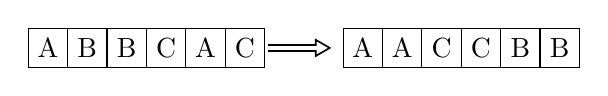
\begin{tikzpicture}[scale=1]
\draw (0,0.0) +(-.25,-.25) rectangle ++(.25,.25);
\draw (0,0.0) node{A};
\draw (0.5,0) +(-.25,-.25) rectangle ++(.25,.25);
\draw (0.5,0) node{B};
\draw (1.0,0) +(-.25,-.25) rectangle ++(.25,.25);
\draw (1.0,0) node{B};
\draw (1.5,0) +(-.25,-.25) rectangle ++(.25,.25);
\draw (1.5,0) node{C};
\draw (2.0,0) +(-.25,-.25) rectangle ++(.25,.25);
\draw (2.0,0) node{A};
\draw (2.5,0) +(-.25,-.25) rectangle ++(.25,.25);
\draw (2.5,0) node{C};

\visible<2-3>
{
\draw[vecArrow] (2.8,0) to (3.6,0);

\draw (4,0.0) +(-.25,-.25) rectangle ++(.25,.25);
\draw (4,0.0) node{A};
\draw (4.5,0) +(-.25,-.25) rectangle ++(.25,.25);
\draw (4.5,0) node{A};
\draw (5.0,0) +(-.25,-.25) rectangle ++(.25,.25);
\draw (5.0,0) node{C};
\draw (5.5,0) +(-.25,-.25) rectangle ++(.25,.25);
\draw (5.5,0) node{C};
\draw (6.0,0) +(-.25,-.25) rectangle ++(.25,.25);
\draw (6.0,0) node{B};
\draw (6.5,0) +(-.25,-.25) rectangle ++(.25,.25);
\draw (6.5,0) node{B};
}
\end{tikzpicture}
\end{figure}

\visible<3>
{
Important features:

\begin{itemize}
\item Airplane only has 1 long row of seats.
\item All family members identical.
\item No preferred sort order (ABC as good as CAB).
\item Can only swap 2 passengers at a time.
\end{itemize}
}
\end{frame}

\begin{frame}\frametitle{Hardness}
Given a set of $n = 3m$ integers $x_i$, is there a grouping of the $x_i$ into $m$ disjoint triplets so that the sum of each triplet is the same number $k$?  

Gadgets:
\visible<2->
{
Large blocking families $B_j$ between each $k$-width seating area.
}

\visible<3->
{
A family of $f_i$ with $x_i$ members for each $x_i$.
}

\visible<4->
{
One seatwarmer family $S$ at end of plane.
}


Starting position:

\begin{figure}[H]
\centering
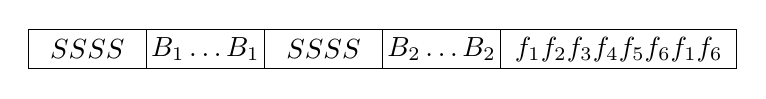
\begin{tikzpicture}[scale=1]
\draw (0,0.0) +(-.75,-.25) rectangle ++(.75,.25);
\visible<4->
{
\draw (0,0.0) node{$SSSS$};
}
\draw (1.5,0) +(-.75,-.25) rectangle ++(.75,.25);
\visible<2->
{
\draw (1.5,0) node{$B_1 \hdots B_1$};
}
\draw (3,0) +(-.75,-.25) rectangle ++(.75,.25);
\visible<4->
{
\draw (3,0) node{$SSSS$};
}
\draw (4.5,0) +(-.75,-.25) rectangle ++(.75,.25);
\visible<2->
{
\draw (4.5,0) node{$B_2 \hdots B_2$};
}
\draw (6.75,0) +(-1.5,-.25) rectangle ++(1.5,.25);
\visible<3->
{
\draw (6.75,0) node{$f_1 f_2 f_3 f_4 f_5 f_6 f_1 f_6$};
}
\end{tikzpicture}
\end{figure}

Final position (only achieveable in $mk$ swaps if there is a 3-partition)

\begin{figure}[H]
\centering
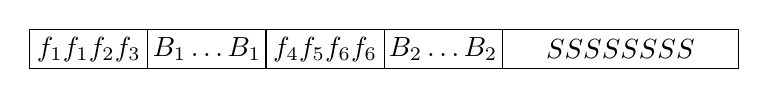
\begin{tikzpicture}[scale=1]
\draw (0,0.0) +(-.75,-.25) rectangle ++(.75,.25);
\visible<3->
{
\draw (0,0.0) node{$f_1 f_1 f_2 f_3$};
}
\draw (1.5,0) +(-.75,-.25) rectangle ++(.75,.25);
\visible<2->
{
\draw (1.5,0) node{$B_1 \hdots B_1$};
}
\draw (3,0) +(-.75,-.25) rectangle ++(.75,.25);
\visible<3->
{
\draw (3,0) node{$f_4 f_5 f_6 f_6$};
}
\draw (4.5,0) +(-.75,-.25) rectangle ++(.75,.25);
\visible<2->
{
\draw (4.5,0) node{$B_2 \hdots B_2$};
}
\draw (6.75,0) +(-1.5,-.25) rectangle ++(1.5,.25);
\visible<4->
{
\draw (6.75,0)node{$SSSSSSSS$};
}
\end{tikzpicture}
\end{figure}

\end{frame}

\begin{frame}{Greedy Algorithm}

We showed that, for a plane filled with couples, the simplest sweep algorithm is optimal due to the following observation:

\begin{figure}[H]
\centering
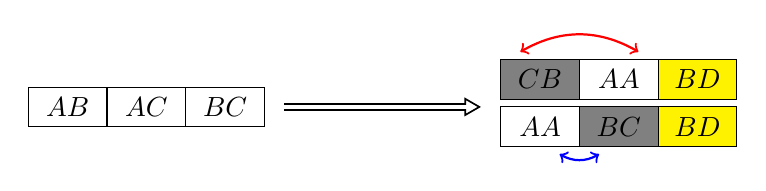
\begin{tikzpicture}[scale=1]
\draw (-6.0,0.25) +(-.5,-.25) rectangle ++(.5,.25);
\draw (-6.0,0.25) node{$A B$};x
\draw (-5.0,0.25) +(-.5,-.25) rectangle ++(.5,.25);
\draw (-5.0,0.25) node{$A C$};
\draw (-4.0,0.25) +(-.5,-.25) rectangle ++(.5,.25);
\draw (-4.0,0.25) node{$B C$};

\draw[vecArrow] (-3.25,0.25) to (-0.75,0.25);

\visible<2>
{
      \draw [thick,red,bend left,<->] (-0.25,0.95) to (1.25,0.95);
}

\visible<4->
    {
      \fill[gray] (0.0,.60) +(-.5,-.25) rectangle ++(.5,.25);
      \fill[gray] (1.0,0) +(-.5,-.25) rectangle ++(.5,.25);

      \fill[yellow] (2.0,.60) +(-.5,-.25) rectangle ++(.5,.25);
      \fill[yellow] (2.0,0) +(-.5,-.25) rectangle ++(.5,.25);

    }

\visible<2->
    {
       \draw (0.0,.60) +(-.5,-.25) rectangle ++(.5,.25);
       \draw (0.0,.60) node{$C B$};
       \draw (1.0,.60) +(-.5,-.25) rectangle ++(.5,.25);
       \draw (1.0,.60) node{$A A$};
       \draw (2.0,.60) +(-.5,-.25) rectangle ++(.5,.25);
       \draw (2.0,.60) node{$B D$};
    }
\visible<3>
{
      \draw [thick,blue,bend right,<->]  (0.25,-0.35) to (0.75,-0.35);
}
\visible<3->
    {
      \draw (0,0.0) +(-.5,-.25) rectangle ++(.5,.25);
      \draw (0,0.0) node{$A A$};
      \draw (1.0,0) +(-.5,-.25) rectangle ++(.5,.25);
      \draw (1.0,0) node{$B C$};
      \draw (2.0,0) +(-.5,-.25) rectangle ++(.5,.25);
      \draw (2.0,0) node{$B D$};
    }
\end{tikzpicture}
\end{figure}

\only<2>
{
The {\color{red}{red} exchange.}
}

\only<3>
{
And the {\color{blue}{blue} exchange.}
}

\only<4>
{
Leave the remaining passengers' seating locations equivalent.
}


\end{frame}

\begin{frame}\frametitle{Mixed Couples and Singles: Alignment}



\begin{figure}[H]
\centering
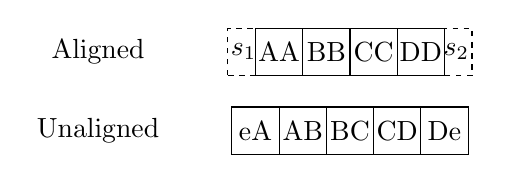
\begin{tikzpicture}[scale=1]
\draw (-2,1) node{Aligned};
\draw[dash pattern= on 2pt off 2pt] (-0.15,1) +(-.2,-.3) rectangle ++(.15,.3);
\draw (-0.15,1) node{$s_1$};
\draw (0.3,1) +(-.3,-.3) rectangle ++(.3,.3);
\draw (0.3,1) node{AA};
\draw (0.9,1) +(-.3,-.3) rectangle ++(.3,.3);
\draw (0.9,1) node{BB};
\draw (1.5,1) +(-.3,-.3) rectangle ++(.3,.3);
\draw (1.5,1) node{CC};
\draw (2.1,1) +(-.3,-.3) rectangle ++(.3,.3);
\draw (2.1,1) node{DD};
\draw[dash pattern= on 2pt off 2pt] (2.55,1) +(-.15,-.3) rectangle ++(.2,.3);
\draw (2.55,1) node{$s_2$};

\draw (-2,0) node{Unaligned};
\draw (0.0,0) +(-.3,-.3) rectangle ++(.3,.3);
\draw (0.0,0) node{eA};
\draw (0.6,0) +(-.3,-.3) rectangle ++(.3,.3);
\draw (0.6,0) node{AB};
\draw (1.2,0) +(-.3,-.3) rectangle ++(.3,.3);
\draw (1.2,0) node{BC};
\draw (1.8,0) +(-.3,-.3) rectangle ++(.3,.3);
\draw (1.8,0) node{CD};
\draw (2.4,0) +(-.3,-.3) rectangle ++(.3,.3);
\draw (2.4,0) node{De};
\end{tikzpicture}
\end{figure}
\end{frame}

\section[DNA]{Genetic Intervals}
\begin{frame}[t]{DNA Copy Analysis}
  \begin{figure}[H] 
    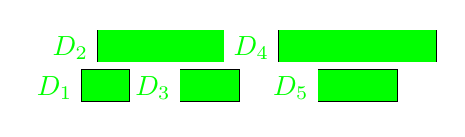
\begin{tikzpicture}[scale=1]

      % We want 5 rectangles that look like:
      %     2222222222       4444444444444444
      % 1111111   33333333       55555555
      \draw (0,0) rectangle (.6,.4);
      \fill[green] (0,0) rectangle (.6,.4);
      \node[green] at (0,-.1) [above left] {$D_1$};

      \draw (.2,.5) rectangle (1.8,.9);
      \fill[green] (.2,.5) rectangle (1.8,.9);
      \node[green] at (.2,.4) [above left] {$D_2$};

      \draw (1.25,0) rectangle (2,.4);
      \fill[green] (1.25,0) rectangle (2,.4);
      \node[green] at (1.25,-.1) [above left] {$D_3$};

      \draw (2.5,.5) rectangle (4.5,.9);
      \fill[green] (2.5,.5) rectangle (4.5,.9);
      \node[green] at (2.5,.4) [above left] {$D_4$};

      \draw (3,0) rectangle (4,.4);
      \fill[green] (3,0) rectangle (4,.4);
      \node[green] at (3,-.1) [above left] {$D_5$};

    \end{tikzpicture} 
    \caption{Simple 5 defect example}
  \end{figure}

  \begin{itemize}
  \item Cancer patients' genomes are 1D objects, i.e. lines.
  \item Closed intervals along that line have genetic abnormalities, and are labeled ``defects.''
  \item Goal: Across a number of patients, identify the $k$ most promising common regions.
  \end{itemize}


\end{frame}

\begin{frame}[t]{Explaining / Scoring}
  \begin{figure}[H] 
    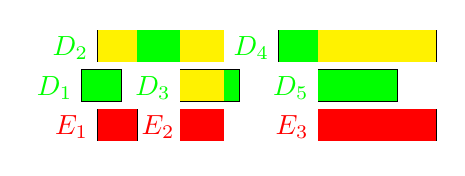
\begin{tikzpicture}[scale=1]

      % We want 5 rectangles that look like:
      %     2222222222       4444444444444444
      % 1111111   33333333       55555555
      \draw (0,0) rectangle (.5,.4);
      \fill[green] (0,0) rectangle (.5,.4);
      \node[green] at (0,-.1) [above left] {$D_1$};

      \draw (.2,.5) rectangle (1.8,.9);
      \fill[green] (.2,.5) rectangle (1.8,.9);
      \node[green] at (.2,.4) [above left] {$D_2$};

      \draw (1.25,0) rectangle (2,.4);
      \fill[green] (1.25,0) rectangle (2,.4);
      \node[green] at (1.25,-.1) [above left] {$D_3$};

      \draw (2.5,.5) rectangle (4.5,.9);
      \fill[green] (2.5,.5) rectangle (4.5,.9);
      \node[green] at (2.5,.4) [above left] {$D_4$};

      \draw (3,0) rectangle (4,.4);
      \fill[green] (3,0) rectangle (4,.4);
      \node[green] at (3,-.1) [above left] {$D_5$};

      %Now draw some explanations

      %% Extends past D_1, scoring only on D_2
      \draw (.2,-.5) rectangle (.7,-.1);
      \fill[red] (.2,-.5) rectangle (.7,-.1);
      \node[red] at (.2,-.6) [above left] {$E_1$};

      \fill[yellow] (.2,.5) rectangle (.7,.9);

      % Overlape D_2 and D_3
      \draw (1.25,-.5) rectangle (1.8,-.1);
      \fill[red] (1.25,-.5) rectangle (1.8,-.1);
      \node[red] at (1.3,-.6) [above left] {$E_2$};

      \fill[yellow] (1.25,.5) rectangle (1.8,.9);
      \fill[yellow] (1.25,0) rectangle (1.8,.4);
      %% Extends past D_5, scoring only on D_4
      \draw (3,-.5) rectangle (4.5,-.1);
      \fill[red] (3,-.5) rectangle (4.5,-.1);
      \node[red] at (3,-.6) [above left] {$E_3$};

      \fill[yellow] (3,.5) rectangle (4.5,.9);

    \end{tikzpicture}
  \end{figure}

  \only<1>{
    Given a set $D$ of defects, find a set $E$ of $k$ closed intervals, or \textit{explanations}, maximizing:

    \begin{equation*}
      \sum_{D_j \in D}  \Big|\bigcup_{(E_i \in E) \cap (E_i \subseteq D_j)} E_i \Big| \frac{1}{|D_j|}
    \end{equation*}
  }

  \only<2->{
    \begin{itemize}
    \item An explanation explains a defect iff it is a subset of that defect.
    \item A specific region of a defect can only be explained once.
    \item An explanation can explain portions of multiple defects.
    \item A defect can be explained by multiple explanations.
    \item Maximum score per defect is 1.
    \end{itemize}
  }

\end{frame}

\begin{frame}{Maximal Explanations}

  \only<1>{
    How many explanations do we have to consider when finding the optimal set?  
  }

  \only<2>{
    The explanation $E_1$ only explains $D_1$, but better scoring explanations exist which also explain $D_1$.
  }

  \only<3>{
    The new explanation $E_2$ is formed by moving the left endpoint of $E_1$ until it matches the left endpoint of $D_1$.
  }

  \only<4>{
    We further improve $E_3$ to become a maximal explanation by making its right endpoint match the right endpoint of $D_1$.
  }

  \only<5>{
    The explanation $E_4$ is trivially non-maximal: it does not explain any defect at all.
  }

  \only<6>{
    $E_5$ is also maximal: its left endpoint is the left endpoint of $D_3$ and its right endpoint matches $D_6$.
  }

  \only<7>{
    Maximal explanations start and end at defect endpoints.  There are $O(n^2)$ maximal explanations for any defect set.
  }

  \begin{figure}[H]
    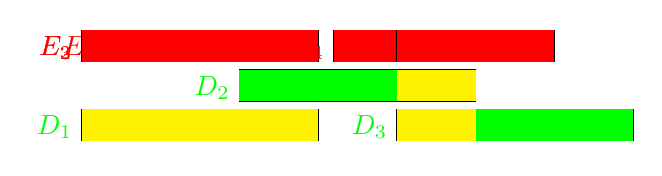
\begin{tikzpicture}[scale=1]

      \uncover<1-> {
        \draw (0,0) rectangle (3,.4);
        \fill[green] (0,0) rectangle (3,.4);
        \node[green] at (0,-.1) [above left] {$D_1$};

        \draw (2,.5) rectangle (5,.9);
        \fill[green] (2,.5) rectangle (5,.9);
        \node[green] at (2,.4) [above left] {$D_2$};

        \draw (4,0) rectangle (7,.4);
        \fill[green] (4,0) rectangle (7,.4);
        \node[green] at (4,-.1) [above left] {$D_3$};
      }

      \uncover<2> {

        \draw (.3,1) rectangle (2.3,1.4);
        \fill[red] (0.3,1) rectangle (2.3,1.4);
        \node[red] at (0.3,.9) [above left] {$E_1$};

        \fill[yellow] (.3,0) rectangle (2.3,.4);
      }

      \uncover<3>  {

        \draw (0,1) rectangle (2.3,1.4);
        \fill[red] (0,1) rectangle (2.3,1.4);
        \node[red] at (0,.9) [above left] {$E_2$};

        \fill[yellow] (0,0) rectangle (2.3,.4);
      }

      \uncover<4,7-> {

        \draw (0,1) rectangle (3,1.4);
        \fill[red] (0,1) rectangle (3,1.4);
        \node[red] at (0,.9) [above left] {$E_3$};

        \fill[yellow] (0,0) rectangle (3,.4);
      }

      \uncover<5> {

        \draw (3.2,1) rectangle (6,1.4);
        \fill[red] (3.2,1) rectangle (6,1.4);
        \node[red] at (3.2,.9) [above left] {$E_4$};
      }

      \uncover<6-> {

        \draw (4,1) rectangle (5,1.4);
        \fill[red] (4,1) rectangle (5,1.4);
        \node[red] at (4,.9) [above left] {$E_5$};

        \fill[yellow] (4,0) rectangle (5,.4);
        \fill[yellow] (4,.5) rectangle (5,.9);
      }

    \end{tikzpicture}
  \end{figure}

\end{frame}

\begin{frame}[t]{Greedy Algorithm}

  \begin{figure}[H]
    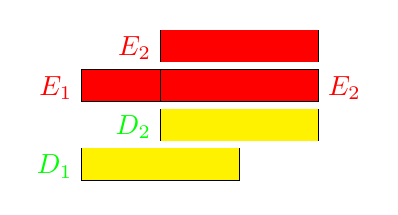
\begin{tikzpicture}[scale=1]

      % We want
      %     2222222222
      % 1111111


      \uncover<1->{
        \draw (0,0) rectangle (2,.4);
        \fill[green] (0,0) rectangle (2,.4);
        \node[green] at (0,-.1) [above left] {$D_1$};

        \draw (1,.5) rectangle (3,.9);
        \fill[green] (1,.5) rectangle (3,.9);
        \node[green] at (1,.4) [above left] {$D_2$};
      }

      \uncover<2>{
        \draw (0,1) rectangle (2,1.4);
        \fill[red] (0,1) rectangle (2,1.4);
        \node[red] at (0,.9) [above left] {$E_1$};


        \draw (1,1.5) rectangle (3,1.9);
        \fill[red] (1,1.5) rectangle (3,1.9);
        \node[red] at (1,1.4) [above left] {$E_2$};

        \fill[yellow] (0,0) rectangle (2,.4);
        \fill[yellow] (1,.5) rectangle (3,.9);  
      }

      \uncover<3->{
        \draw (1,1) rectangle (2,1.4);
        \fill[red] (1,1) rectangle (2,1.4);
        \node[red] at (1,.9) [above left] {$E_3$};

        \fill[yellow] (1,0) rectangle (2,.4);
        \fill[yellow] (1,.5) rectangle (2,.9);
        
      }

      \uncover<4->{
        \draw (2,1) rectangle (3,1.4);
        \fill[red] (2,1) rectangle (3,1.4);
        \node[red] at (3,.9) [above right] {$E_2$};

        \fill[yellow] (2,.5) rectangle (3,.9);
        
      }
    \end{tikzpicture} 
  \end{figure}

  This is the simplest example where Greedy is non-optimal:

  \only<2>{
    When we allow 2 explanations to cover 2 defects, the obvious correct answer is $E_1 = D_1$ and $E_2 = D_2$.
  }

  \only<3->{
    However, in the first step of greedy, we select the high scoring center region.
  }

  \only<4->{
    This leaves us with lower scoring side regions for our next selection.  Greedy only scored $\frac34$ of the maximum attainable score by making a bad first selection.
  }
\end{frame}

\begin{frame}[t]{1-OPT Exchange Algorithm}

  \begin{figure}[H]
    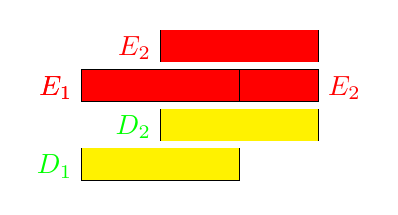
\begin{tikzpicture}[scale=1]

      % We want
      %     2222222222
      % 1111111


      \draw (0,0) rectangle (2,.4);
      \fill[green] (0,0) rectangle (2,.4);
      \node[green] at (0,-.1) [above left] {$D_1$};

      \draw (1,.5) rectangle (3,.9);
      \fill[green] (1,.5) rectangle (3,.9);
      \node[green] at (1,.4) [above left] {$D_2$};

      \uncover<1,2,3>{
        \draw (1,1) rectangle (2,1.4);
        \fill[red] (1,1) rectangle (2,1.4);

        \fill[yellow] (1,0) rectangle (2,.4);
        \fill[yellow] (1,.5) rectangle (2,.9);
      }

      \uncover<1,2>  {
        \node[red] at (1,.9) [above left] {$E_3$};
      }
      
      \uncover<1>  {
        \draw (2,1) rectangle (3,1.4);
        \fill[red] (2,1) rectangle (3,1.4);
        \node[red] at (3,.9) [above right] {$E_2$};

        \fill[yellow] (2,.5) rectangle (3,.9);
        
      }

      \uncover<3>{
        % Fix label covered in step 3 by $E_1$
        \node[red] at (2,.9) [above right] {$E_3$};
      }

      \uncover<3,4> {
        \draw (0,1) rectangle (2,1.4);
        \fill[red] (0,1) rectangle (2,1.4);
        \node[red] at (0,.9) [above left] {$E_1$};
        \fill[yellow] (0,0) rectangle (2,.4);

      }

      \uncover<5->{
        \draw (0,1) rectangle (2,1.4);
        \fill[red] (0,1) rectangle (2,1.4);
        \node[red] at (0,.9) [above left] {$E_1$};


        \draw (1,1.5) rectangle (3,1.9);
        \fill[red] (1,1.5) rectangle (3,1.9);
        \node[red] at (1,1.4) [above left] {$E_2$};

        \fill[yellow] (0,0) rectangle (2,.4);
        \fill[yellow] (1,.5) rectangle (3,.9);  
      }
    \end{tikzpicture} 
  \end{figure}

  \only<1>{
    We illustrate 1-OPT with the $n=k=2$ worst case defect set from before.  1-OPT starts with the greedy solution.
  }

  \only<2,3>{
    It then removes each explanation in turn ($E_2$ in this case) and tries to replace it with an explanation that scores at least as much.
  }

  \only<3>{
    Here $E_1$ was selected to replace $E_2$.
  }

  \only<4,5> {
    Now we remove $E_3$ to try and improve the score.
  }

  \only<5> {
    The best scoring maximal explanation remaining is $E_2$.
  }

  \only<6> {
    We test to see if removing an explanation and replacing it can further improve the score.  Since it cannot, the algorithm terminates.
  }

\end{frame}

\begin{frame}[t]{1-OPT Isn't Optimal}

  \begin{figure}[H]
    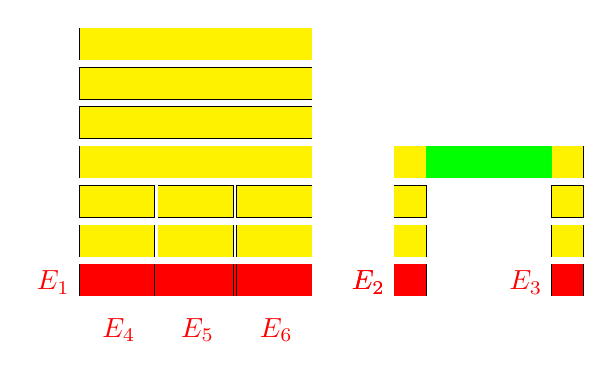
\begin{tikzpicture}[scale=1]

      % 6 small rectangles on the left in 2 rows of 3
      \foreach \x in {0,1,2} {
        \foreach \y in {0,1} {
          \draw (0+\x,0+\y/2) rectangle (.95+\x,.4+\y/2);
          \fill[green] (0+\x,0+\y/2) rectangle (.95+\x,.4+\y/2);
        }
      }
      
      % 4 Wide caps on those small rectangles
      \foreach \y in {0,1,2,3} {
        \draw (0,1+\y/2) rectangle (2.95,1.4+\y/2);
        \fill[green] (0,1+\y/2) rectangle (2.95,1.4+\y/2);
      }

      
      \foreach \y in {0,1} {
        \foreach \x in {4, 6} {
          \draw (0+\x,0+\y/2) rectangle (.4+\x,.4+\y/2);
          \fill[green] (0+\x,0+\y/2) rectangle (.4+\x,.4+\y/2);
        }
      }                  
      \draw (4,1) rectangle (6.4,1.4);
      \fill[green] (4,1) rectangle (6.4,1.4);

      \uncover<2,4,6>{
        \draw (0,-.5) rectangle (2.95, -.1);
        \fill[red] (0,-.5) rectangle (2.95, -.1);
        \node[red] at (0,-.6) [above left] {$E_1$};
        \foreach \y in {0,1,2,3} {
          \fill[yellow] (0,1+\y/2) rectangle (2.95,1.4+\y/2);
        }
      } %uncover<2.4>

      \uncover<2,4,5>{
        \draw (4,-.5) rectangle (4.4, -.1);
        \fill[red] (4,-.5) rectangle (4.4, -.1);
        \node[red] at (4,-.6) [above left] {$E_2$};
        
        \draw (6,-.5) rectangle (6.4, -.1);
        \fill[red] (6,-.5) rectangle (6.4, -.1);
        \node[red] at (6,-.6) [above left] {$E_3$};

        
        \foreach \y in {0,1,2} {
          \foreach \x in {4, 6} {
            \fill[yellow] (0+\x,0+\y/2) rectangle (.4+\x,.4+\y/2);
          }
        }                                               
      } % uncover<2,4,5>

      \uncover<6>{
        \foreach \y in {0,1,2} {
          \fill[yellow] (4,0+\y/2) rectangle (4.4,.4+\y/2);
        }
        \draw (4,-.5) rectangle (4.4, -.1);
        \fill[red] (4,-.5) rectangle (4.4, -.1);
        \node[red] at (4,-.6) [above left] {$E_2$};

      }

      \uncover<3,7>{
        \foreach \x in {4,5,6} {
          \draw (-4+\x,-.5) rectangle (-3.05+\x,-.1);
          \fill[red] (-4+\x,-.5) rectangle (-3.05+\x,-.1);
          \node[red] at (-3.5+\x,-1.2) [above] {$E_\x$};
        }

        \foreach \x in {0,1,2} {
          \foreach \y in {0,1} {
            \fill[yellow] (0+\x,0+\y/2) rectangle (.95+\x,.4+\y/2);
          }
        }
        \foreach \y in {0,1,2,3} {
          \fill[yellow] (0,1+\y/2) rectangle (2.95,1.4+\y/2);
        }
      } % uncover 3
      
    \end{tikzpicture}
  \end{figure}          

  \only<1>{  
    Our starting defect set has a number of identical defects.  

    We are going to explain these 15 defects with 3 explanations. 
  }

  \only<2>{
    This is our bad solution.

    $E_1$ scores 4.

    Both $E_2$ and $E_3$ score $2+\epsilon$.

    For a total of $8 + 2\epsilon$.
  }

  \only<3>{
    This is the optimal solution.

    Each of $E_4, E_5$ and $E_6$ score $3 \frac13$.

    This total of $10$ beats our bad solution.
  }

  \only<4,5,6>{
    Unfortunately, there is no good option for removal from the bad case.
  }

  \only<5>{
    Without $E_1$ in place, $E_4, E_5$ and $E_6$ only score $3 \frac13$, which is lower than $E_1$'s score of 4.
  }

  \only<6>{
    When $E_3$ is offered for exchange, $E_4, E_5$ and $E_6$ only score $2$ which is less than the $2+\epsilon$ that $E_3$ had scored.
  }

  \only<7>{
    Unfortunately, this optimal arrangement cannot be reached from the starting point we chose.

    This means that 1-OPT is not guaranteed to be optimal for $n>k$.
  }

\end{frame}

\begin{frame}[t]{Dynamic Programming PTAS}

\begin{figure}[ht!] \centering
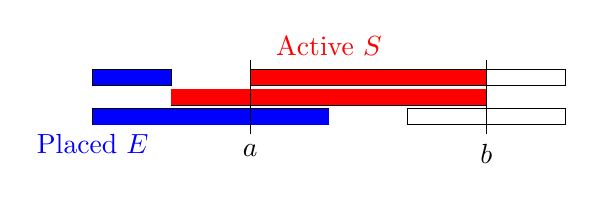
\begin{tikzpicture}[xscale=1,yscale=.25]

\draw (4,0) rectangle (6,0.8);

\draw (1,1) rectangle (5,1.8);
\fill[red] (1,1) rectangle (5,1.8);

\node[red] at (3,3) [above] {Active $S$};

\draw (2,2) rectangle (6,2.8);
\fill[red] (2,2) rectangle (5,2.8);

\draw (0,0) rectangle (3,0.8);
\fill[blue] (0,0) rectangle (3,0.8);

\draw (0,2) rectangle (1,2.8);
\fill[blue] (0,2) rectangle (1,2.8);

\node[blue] at (0,0) [below] {Placed $E$};


\draw (2,-.5) -- (2,3.3);
\node[black] at (2,-.5) [below] {$a$};

\draw (5,-.5) -- (5,3.3);
\node[black] at (5,-.5) [below] {$b$};

\end{tikzpicture} 
\end{figure}

\end{frame}

\begin{frame}[t]{DP Updates}

\begin{figure}[ht!] \centering
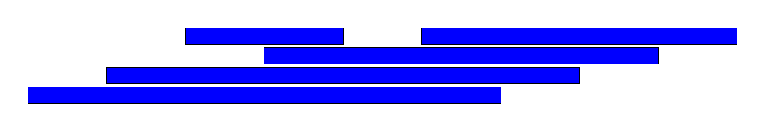
\begin{tikzpicture}[xscale=1,yscale=.25]

\coordinate (L1) at (1,0);
\coordinate (R1) at (7,0.8);

\coordinate (L2) at (2,1);
\coordinate (R2) at (8,1.8);

\coordinate (L3) at (4,2);
\coordinate (R3) at (9,2.8);

\coordinate (L4) at (6,3);
\coordinate (R4) at (10,3.8);

\coordinate (L5) at (3,3);
\coordinate (R5) at (5,3.8);

\foreach \rect in {1,2,3,4,5} {
  \draw (L\rect) rectangle (R\rect);
  \fill[blue] (L\rect) rectangle (R\rect);
}

\end{tikzpicture} 
\end{figure}


\end{frame}

\section[Waiter]{Waiter Problem}
\begin{frame}\frametitle{Don't Drop that Tray}

\end{frame}

\end{document}

